\section{Preparación del Entorno de Construcción}{
\noindent La preparación del entorno de construcción implica la descripción de los puestos de trabajo y la instalación de las herramientas y bibliotecas a usar durante el desarrollo y codificación del proyecto.\\

\noindent Como consideración previa se contempla que las computadoras usadas para el desarrollo deben de poseer el sistema operativo GNU/Linux, específicamente en su distribución Ubuntu.

\subsection{Puestos de trabajo}{
\noindent Para los puestos de trabajo se tiene contemplado hacer uso de 3 computadoras portátiles (1 para cada miembro del equipo de trabajo) las cuales cumplan con lo necesario para poder instalar y hacer uso de las diferentes herramientas y librerías que se especifican en los apartados X y Z respectivamente. Los equipos que con los que actualmente se cuenta son los siguientes:
% Please add the following required packages to your document preamble:
% \usepackage{longtable}
% Note: It may be necessary to compile the document several times to get a multi-page table to line up properly
\begin{longtable}[c]{lllll}
\cline{1-2}
\multicolumn{1}{|l|}{\textbf{Equipo}}           & \multicolumn{1}{l|}{\textbf{Especificaciones Técnicas}}                                                                                                                                                                                                                                    &  &  &  \\ \cline{1-2}
\endfirsthead
%
\multicolumn{5}{c}%
{{\bfseries Table \thetable\ continued from previous page}} \\
\endhead
%
\multicolumn{1}{|l|}{HP Notebook - 15-ac128la}  & \multicolumn{1}{l|}{\begin{tabular}[c]{@{}l@{}}°Procesador Intel Core i7-6500U (2,5 GHz,\\     hasta 3,1 GHz, 4 MB de caché, 2 núcleos).\\ Memoria RAM de 8GB\\ Gráficos de video Intel HD 520\\ Disco Duro SATA de 2TB 5400 rpm\end{tabular}}                                          &  &  &  \\ \cline{1-2}
\multicolumn{1}{|l|}{HP Pavilion Laptop 15-cw0} & \multicolumn{1}{l|}{\begin{tabular}[c]{@{}l@{}}Procesador AMD Ryzen 3 con \\    gráficos Radeon Vega Graphics \\    Mobile Gfx (Cuatro núcleos a 3,4 GHz \\    en modo base y 3,7 GHz en modo turbo).\\ Memoria RAM de 12GB.\\ Disco Duro SSD SATA3 de 500 GB.\end{tabular}}           &  &  &  \\ \cline{1-2}
\multicolumn{1}{|l|}{Lenovo Ideapad 110-14 ISK} & \multicolumn{1}{l|}{\begin{tabular}[c]{@{}l@{}}°Procesador Intel Core i7-649DU (2,5 GHz, \\   hasta 3,1 GHz, 4 MB de caché, 4 núcleos).\\ Memoria RAM de 8GB .Disco Duro Toshiba\\    MQ01 de 1TB.Disco Duro Kingston SSD \\    de 240 GB.\\ °Gráficos de video Intel HD510\end{tabular}} &  &  &  \\ \cline{1-2}
                                                &                                                                                                                                                                                                                                                                                            &  &  & 
\end{longtable}
}
\subsection{Herramientas}{
\subsubsection{Visual Studio Code}

\noindent Visual Studio Code es un editor de código fuente desarrollado por \textbf{Microsoft} y este puede ser utilizado en los Sistemas Operativos \textbf{Linux}, \textbf{macOS} y obviamente \textbf{Windows}. Esta herramienta cuenta con diversas funciones útiles para nosotros, algunas de ellas son:

\begin{itemize}
    \item Soporte de Depuración.
    \item Control de versiones por Git.
    \item Resaltado de sintaxis.
    \item Finalización inteligente de código.
\end{itemize}
\noindent Este editor, nos ofrece otra ventaja al ser gratuito y de código abierto, ignorando el hecho de que la descarga está bajo la licencia de software por el propietario.\\

\noindent La descarga se puede hacer desde la página:
\hyperlink{https://code.visualstudio.com/Download}{https://code.visualstudio.com/Download} en el apartado correspondiente al paquete .deb, lo anterior ilustrado por la figura \ref{2.1.1}.

\begin{figure}[H]
    \centering
    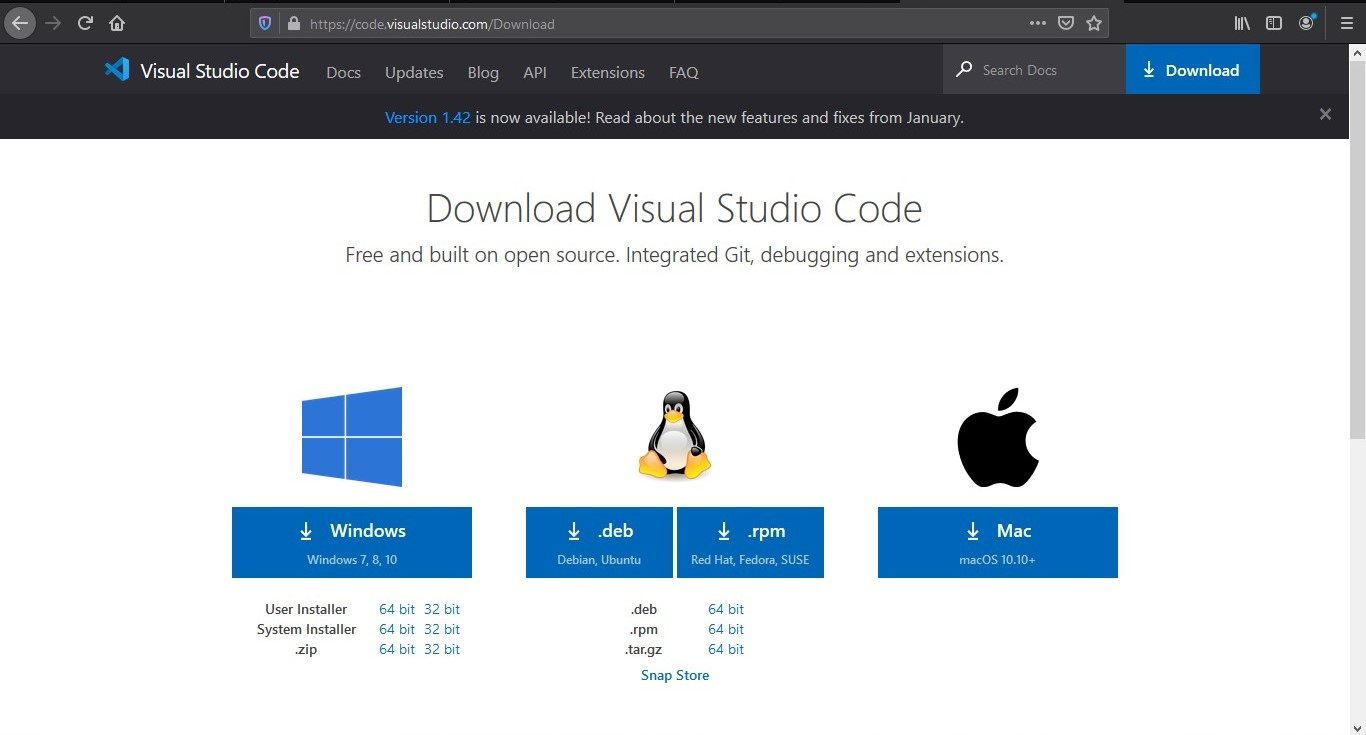
\includegraphics[scale=0.5]{Capitulo4/Documentos/imagenes_entorno/figura2-1-1.jpg}
    \caption{Ventana de descargas del editor Visual Studio Code, con el apartado .deb (paquete para equipos Linux basados en Debian) señalado.}
    \label{2.1.1}
\end{figure}

\noindent Una vez descargado el paquete se recurre a la instalación del .deb que es el requerido para la distribución que tengamos basada en Debian.  El gestor de paquetes de Ubuntu es el que controla la instalación, y para instalar Visual Studio Code se puede utilizar el centro de software de Ubuntu, el cual se muestra de manera automática cuando se hace doble clic sobre el paquete de instalación con extensión .deb. Este proceso identifica la aplicación que se desea instalar y muestra una interfaz al usuario en la que el mismo puede proceder a instalar la aplicación o a cancelar el proceso. La interfaz del centro de software de ubuntu muestra una pantalla como la de la figura \ref{2.1.2} cuando se hace doble clic sobre el paquete descargado previamente.

\begin{figure}[H]
    \centering
    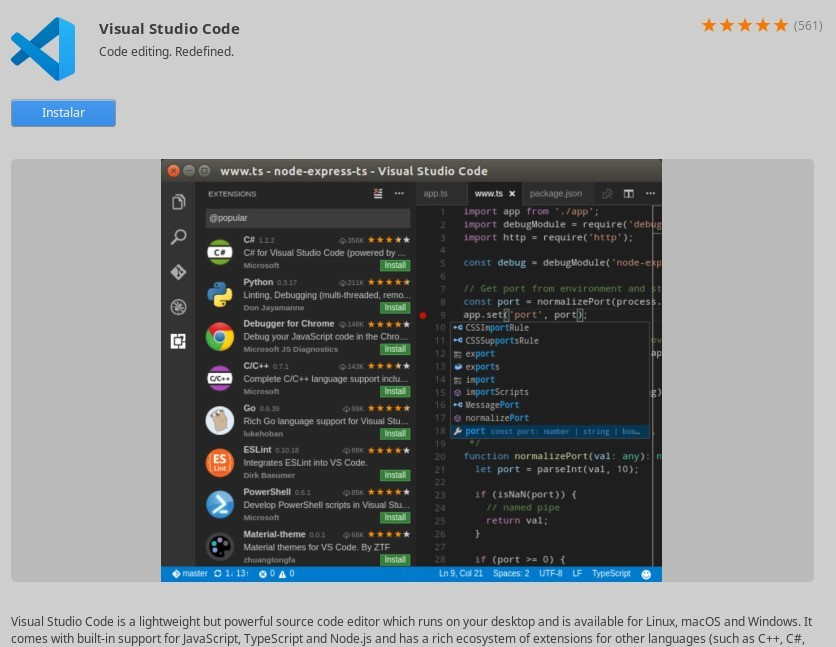
\includegraphics[scale=0.82]{Capitulo4/Documentos/imagenes_entorno/figura2-1-2.jpg}
    \caption{Instalación de Visual Studio Code mediante el centro de software de Ubuntu.}
    \label{2.1.2}
\end{figure}

\noindent Una vez concluida la instalación, para verificar que esta haya ido correctamente, se procede a abrir el editor, el cual debe mostrarse en una pantalla de inicio como la que ilustra la figura \ref{2.1.3}.

\begin{figure}[H]
    \centering
    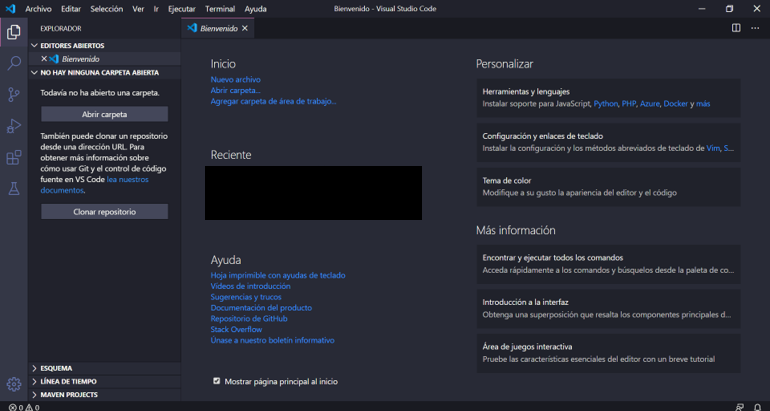
\includegraphics[scale=0.82]{Capitulo4/Documentos/imagenes_entorno/figura2-1-3.png}
    \caption{Ventana de inicio de Visual Studio Code.}
    \label{2.1.3}
\end{figure}

\subsubsection{Python en su versión 3}

\noindent El lenguaje con el que se desarrollará es Python, que para el caso de Ubuntu ya posee una versión de python instalada, para verificar esto se puede ingresar el siguiente comando en la terminal del sistema:
\begin{lstlisting}
python -V
\end{lstlisting}
La figura \ref{2.2.1} muestra el resultado de ejecutar este comando, el cual es el número de versión de python que el sistema tiene instalado en ese momento.

\begin{figure}[H]
    \centering
    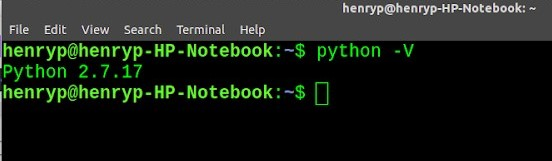
\includegraphics[scale=0.85]{Capitulo4/Documentos/imagenes_entorno/figura2-2-1.jpg}
    \caption{Resultado de la ejecución del comando para obtener la versión de python. En esta imagen se muestra que se tiene instalada la versión 2.7.}
    \label{2.2.1}
\end{figure}
\newpage
\noindent Sin embargo, para el desarrollo del sistema se requiere utilizar python en su versión 3.6.9. Para obtener esta versión en particular, se utiliza terminal para ingresar el siguiente comando:

\begin{lstlisting}
sudo add-apt-repository ppa:deadsnakes/ppa
sudo apt update
sudo apt install python3.6
\end{lstlisting}
\noindent Para corroborar la instalación de python en su versión 3.6.9, se ejecuta el comando:

\begin{lstlisting}
python3 -V
\end{lstlisting}
\noindent en la terminal del sistema. El resultado debe ser idéntico al que se puede ver señalado en la figura \ref{2.2.2}.
\begin{figure}[H]
    \centering
    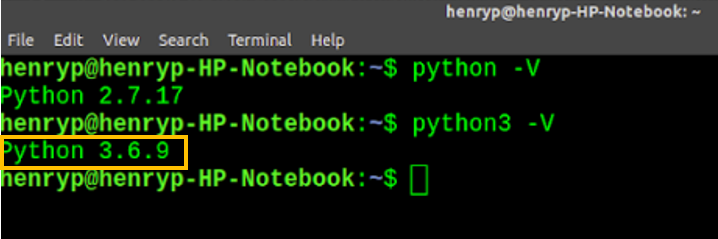
\includegraphics[scale=0.85]{Capitulo4/Documentos/imagenes_entorno/figura2-2-2.png}
    \caption{Verificación de la instalación de la versión correcta de python, se señala el resultado que indica la versión 3.6.9.}
    \label{2.2.2}
\end{figure}

\subsubsection{PIP}\\

\noindent PIP es un sistema de gestión de paquetes utilizado para instalar y administrar paquetes de software escritos en Python.\\

\noindent A partir de la instalación de python en la versión mayor a 3 (en este caso se utiliza la versión 3.6.9), PIP ya viene incluido (pero ahora es denominado PIP3), sin embargo, se puede verificar que ya se encuentra instalado ejecutando el siguiente comando en la terminal:

\begin{lstlisting}
pip3 --version
\end{lstlisting}

\noindent Como resultado de ejecutar este comando en la terminal se debe observar una respuesta del sistema similar a la que muestra la figura \ref{2.3.1}.

\begin{figure}[H]
    \centering
    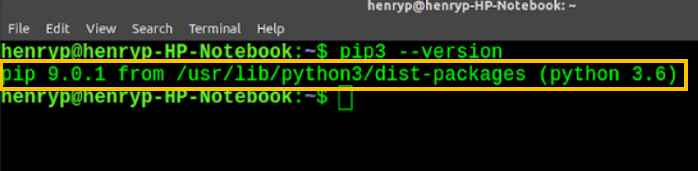
\includegraphics[scale=0.85]{Capitulo4/Documentos/imagenes_entorno/figura2-3-1.png}
    \caption{Comprobación de la instalación de PIP donde el resultado se encuentra señalado (incluso se indica para qué versión de python está configurado pip).}
    \label{2.3.1}
\end{figure}

\subsubsection{ChromeDriver}

\noindent Dado que se pretende trabajar con una biblioteca llamada Selenium, esta última requiere de un driver que sea compatible con el navegador deseado a trabajar, para el desarrollo del sistema de información, se optó por usar el navegador Google Chrome como el navegador predeterminado, para ello requerimos del driver de nombre ChromeDriver.\\

\noindent Antes de la descarga e instalación se deben de cumplir con algunos requisitos, y para instalar en ChromeDriver en el sistema operativo que se está utilizando, se debe empezar por lo ingresar los siguientes dos comandos en la terminal del sistema:
\begin{lstlisting}
sudo apt-get update
sudo apt-get install -z unzip xvfb libx16 libgconf 2-4
\end{lstlisting}

\noindent Posteriormente, se debe actualizar o instalar la versión más actual de Google Chrome, esto es más directo si se recurre a la página de descargas de Chrome, se descarga el .deb y se utiliza dicha herramienta de software para instalarlo.
La figura \ref{2.4.1} muestra la ventana de descargas del navegador. La misma página identifica el sistema operativo cuando se hace clic en el botón “Descargar Chrome”.

\begin{figure}[H]
    \centering
    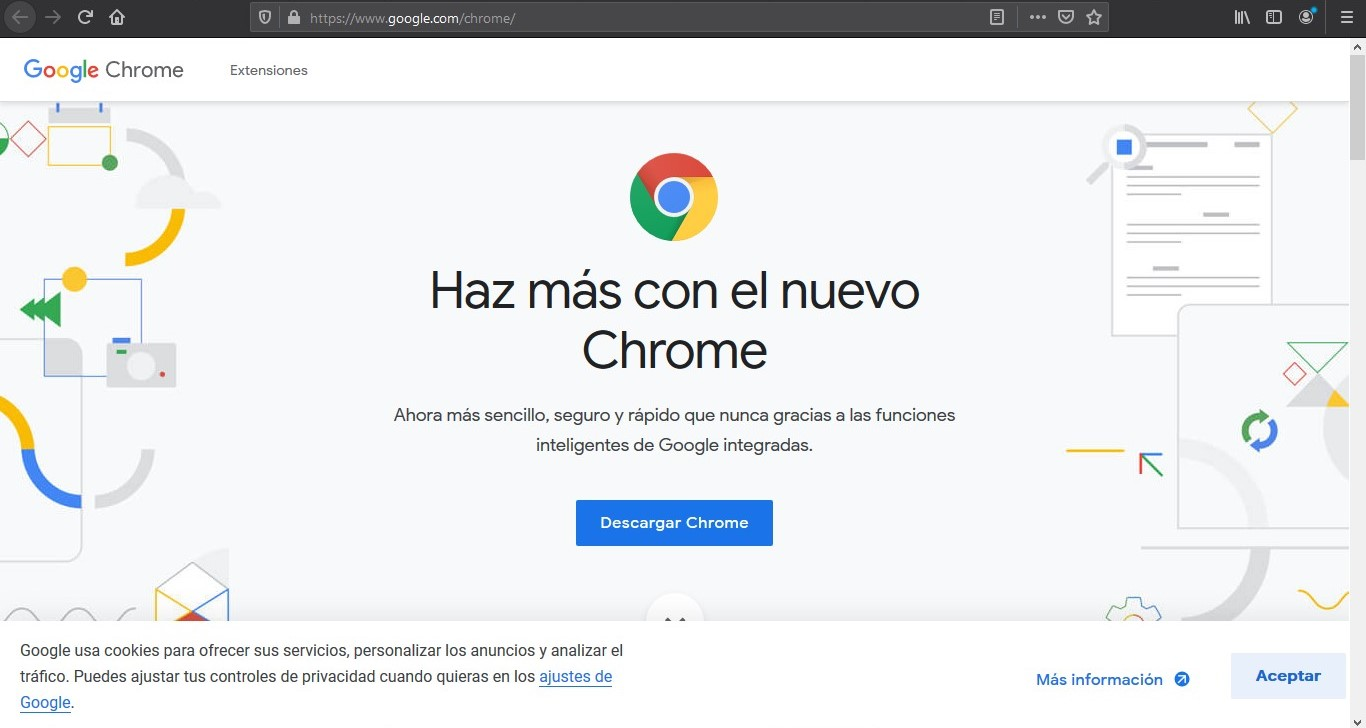
\includegraphics[scale=0.52]{Capitulo4/Documentos/imagenes_entorno/figura2-4-1.jpg}
    \caption{Página de descargas del navegador.}
    \label{2.4.1}
\end{figure}

Ya instalado el navegador, se puede continuar con el driver del navegador, para ello se visita la siguiente página:\\

\href{https://sites.google.com/a/chromium.org/chromedriver/downloads.}{https://sites.google.com/a/chromium.org/chromedriver/downloads.}\\

\noindent La figura \ref{2.4.2} ilustra una vista de la página de descargas descrita previamente.

\begin{figure}[H]
    \centering
    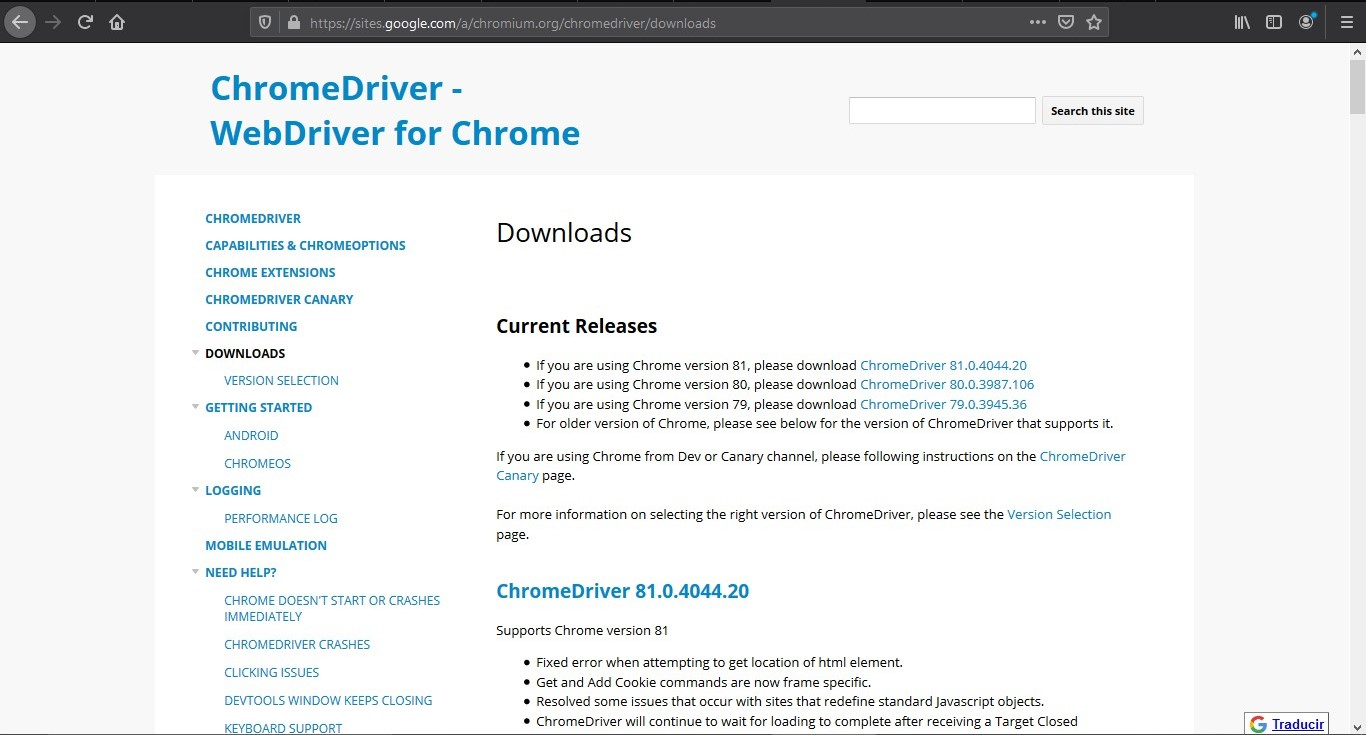
\includegraphics[scale=0.51]{Capitulo4/Documentos/imagenes_entorno/figura2-4-2.jpg}
    \caption{Página de descargas para el driver del navegador.}
    \label{2.4.2}
\end{figure}

\noindent Donde se selecciona el driver, según la versión del navegador Chrome que se tenga instalada, y se descarga el archivo. Ya con el archivo descargado, se obtiene su ubicación donde fue almacenado en el equipo y se hace clic derecho sobre el directorio seguido de la opción “Abrir en la terminal” para desplegar la pantalla de una terminal que ya esté directamente relacionada con la ruta donde se encuentra el archivo., una vez ahí, se ejecutan los siguientes comandos:

\begin{itemize}
    \item Se descomprime el .zip, cabe aclarar que se incluye en el comando, la característica del sistema, es decir los 64 bits.
\end{itemize}

\begin{lstlisting}
unzip chromedriver_linux64.zip  
\end{lstlisting}

\begin{itemize}
    \item Ya que se tiene el contenido, se realiza la instalación en el PATH:
\end{itemize}
\begin{lstlisting}
sudo mv chromedriver /usr/bin/chromedriver
sudo chown root:root /usr/bin/chromedirver
sudo chmod +x /usr/bin/chromedriver
\end{lstlisting}
\noindent Finalizado todo ya se cuenta con el driver necesario para la adquisición de los datos a través del navegador.
}
\\

\subsubsection{MGLTools}

\noindent MGLTools es un software desarrollado en el Laboratorio de Gráficos Moleculares (MGL) del Instituto de Investigación Scripps para la visualización y análisis de estructuras moleculares.
Utilizaremos esta herramienta para la transformación de las estructuras moleculares de los compuestos y las proteínas, esto  con la finalidad de generar receptores que puedan acoplarse a una estructura de un ligando.\\

\noindent Ejecutando la siguiente lista de comandos podremos descargar esta herramienta:
\begin{lstlisting}
wget http://mgltools.scripps.edu/downloads/downloads/tars
/releases/REL1.5.6/mgltools_x86_64Linux2_1.5.6.tar.gz
tar -xzvf mgltools_x86_64Linux2_1.5.6.tar.gz
cd mgltools_x86_64Linux2_1.5.6
./install.sh
cd MGLToolsPckgs/AutoDockTools/Utilities24
sudo cp prepare_ligand4.py /usr/local/bin
sudo cp prepare_receptor4.py /usr/local/bin
sudo cp prepare_gpf4.py /usr/local/bin
cd ../../..
cd bin
sudo cp pythonsh /usr/local/bin
\end{lstlisting}


\subsubsection{AutoDock-Vina}\\

\noindent AutoDock Vina es un conjunto de herramientas de acoplamiento automatizadas. Está diseñado para predecir cómo las moléculas pequeñas, como sustratos o candidatos a fármacos, se unen a un receptor de estructura 3D conocida.\\

\noindent Esta herramienta sera utilizada para realizar un docking más preciso introduciendo las estructuras del ligando y el receptor.
Para realizar su instalación ejecutaremos la siguiente lista de comandos:
\begin{lstlisting}
sudo wget http://vina.scripps.edu/download/autodock_vina_1_1_2_linux_x86.tgz
echo descomprimir
tar -xzvf autodock_vina_1_1_2_linux_x86.tgz
cd autodock_vina_1_1_2_linux_x86/bin
cp vina /usr/local/bin
\end{lstlisting}

\subsubsection{AutoGrid}\\

\noindent AutoGrid es un programa que calcula previamente los mapas de cuadrícula de las energías de interacción para varios tipos de átomos, como los carbonos alifáticos, los carbonos aromáticos, los oxígenos de enlace de hidrógeno, etc., con una macromolécula como una proteína, ADN o ARN.\\

\noindent Estos mapas de cuadrícula se utilizan luego en los cálculos de acoplamiento de AutoDock para determinar la energía de interacción total para un ligando con una macromolécula.

\noindent Para la instalación de esta herramienta, ejecutamos la siguiente lista de comandos en la terminal:
\begin{lstlisting}
sudo wget http://autodock.scripps.edu/downloads/
autodock-registration/tars/dist426/
autodocksuite-4.2.6-x86_64Linux3.tar
echo Descomprimiendo autodocksuite
tar -xvf autodocksuite-4.2.6-x86_64Linux3.tar
cd x86_64Linux3
cp autodock4 /usr/local/bin
cp autogrid4 /usr/local/bin
\end{lstlisting}
\subsection{Bibliotecas}{
\noindent La instalación de bibliotecas se realiza utilizando el administrador de paquetes para python PIP en su versión para python3 el cual corresponde al comando de pip3, cuya instalación se menciona en el apartado X. Es importante señalar que para todas las bibliotecas que se van a instalar se requiere conexión a internet. Para verificar la correcta instalación de cada biblioteca, basta con dar seguimiento a la información que el sistema va mostrando mientras se encuentra instalando la biblioteca especificada. Las bibliotecas aquí descritas cuando han sido correctamente instaladas muestran un mensaje (definido por pip3) como el que se señala en la figura \ref{3.1}, donde se toma como ejemplo la instalación de la biblioteca Requests, y al final puede leerse la frase en inglés “Successfully installed” seguido del nombre completo de la biblioteca.

\begin{figure}[H]
    \centering
    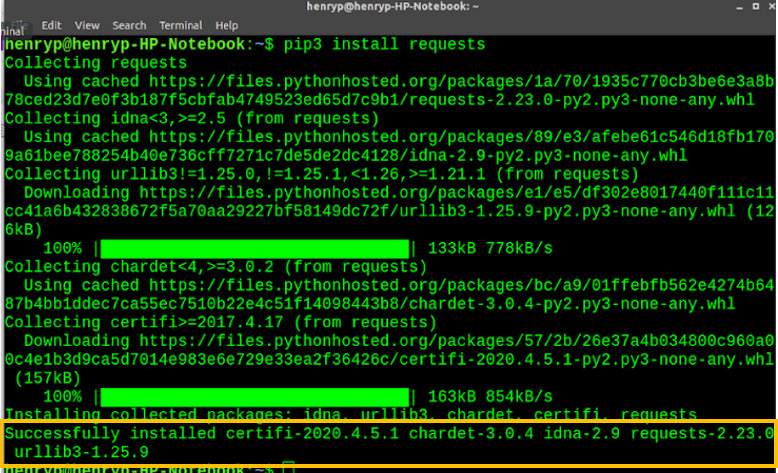
\includegraphics[scale=0.85]{Capitulo4/Documentos/imagenes_entorno/figura3-1.png}
    \caption{Instalación exitosa de la biblioteca Requests, donde se señala el mensaje que arroja pip3 de éxito del proceso de instalación.}
    \label{3.1}
\end{figure}
\subsubsection{Tkinter}\\

\noindent Con Python hay muchas posibilidades para programar una interfaz gráfica de usuario (GUI) pero Tkinter es fácil de usar, es multiplataforma y, además, viene incluido con Python en su versión para Windows, para Mac y para la mayoría de las distribuciones GNU/Linux. Se le considera el estándar de facto en la programación GUI con Python.\\

\noindent Tkinter es un binding de la biblioteca Tcl/Tk que está también disponible para otros lenguajes como Perl y Ruby.
A pesar de su larga historia, su uso no está demasiado extendido entre los usuarios de equipos personales porque su integración visual con los sistemas operativos no era buena y proporcionaba pocos widgets (controles) para construir los programas gráficos.
Para instalar Tkinter se debe escribir y ejecutar el siguiente comando en la terminal:
\begin{lstlisting}
sudo apt-get install python3-tk
\end{lstlisting}
\noindent Para verificar esta instalación, se procede a ingresar a la línea de comandos de python3 simplemente ejecutando en la terminal el comando:
\begin{lstlisting}
python3 
\end{lstlisting}
\noindent Luego se procede a escribir las siguientes dos líneas:
\begin{lstlisting}
import tkinter
tkinter.TkVersion
\end{lstlisting}
\noindent Si la instalación se ha hecho correctamente, la terminal arroja un resultado como el que se señala en la figura \ref{3.1.1}.

\begin{figure}[H]
    \centering
    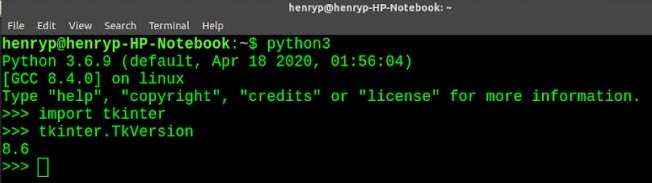
\includegraphics[scale=0.85]{Capitulo4/Documentos/imagenes_entorno/figura3-1-1.jpg}
    \caption{Confirmación de la instalación de Tkinter.}
    \label{3.1.1}
\end{figure}
\subsubsection{Requests}\\

\noindent Requests es una librería de Python para peticiones HTTP liberada bajo una la licencia de Apache License 2.0.  Request permite enviar solicitudes HTTP / 1.1 con extrema facilidad.\\ 

\noindent No es necesario agregar manualmente cadenas de consulta a sus URL, ni codificar de forma estricta los datos POST. Keep-alive y el grupo de conexiones HTTP son 100\% automáticas.\\

\noindent La instalación en Linux es de la siguiente manera. Como ya se ha instalado PIP en la versión para python3, basta con el siguiente comando:\\

\begin{lstlisting}
pip3 install requests
\end{lstlisting}

\subsubsection{Selenium}\\

\noindent Selenium para Python proporcionan una API simple para navegar o realizar pruebas en algún navegador web, utilizando un WebDriver. A través de Selenium Python API puede acceder a todas las funcionalidades de Selenium WebDriver de una manera sencilla e intuitiva.\\
Selenium Python proporcionan una API conveniente para acceder a Selenium WebDrivers como Firefox, Internet Explorer, Chrome, Remote, etc. Y es compatible con versiones de Python desde la 2.7.\\

\noindent
Para la instalación se ejecuta el siguiente comando en la terminal del sistema:
\begin{lstlisting}
pip3 install selenium
\end{lstlisting}

\subsubsection{Pillow}\\

\noindent Es una librería gratuita que permite la edición de imágenes directamente desde Python. Soporta una variedad de formatos, incluidos los más utilizados como GIF, JPEG y PNG. Una gran parte del código está escrito en C, por cuestiones de rendimiento.\\

\noindent Debido a que la librería soporta únicamente hasta la versión 2.7 de Python y, al parecer, no se propuso avanzar con él, un equipo de desarrolladores en colaboración se ha desarrollado Pillow, una bifurcación, con un desarrollo más «amigable», así nace PIL que pretende mantener una librería estable y que se adapte a las nuevas tecnologías (De Python 3 en adelante). Por esta razón, PIL entró en función en lugar de Pillow.\\

\noindent Para proceder con la instalación, se ingresa y ejecuta el siguiente comando en la terminal del sistema:

\begin{lstlisting}
pip3 install Pillow
\end{lstlisting}

\subsubsection{BioPython}

\noindent BioPython es el nombre que recibe una serie de aplicaciones y programas informáticos pensados para cuantificar y hacer cálculos con datos biológicos, programados por una comunidad internacional. El uso de esta biblioteca apoya en aportar el mayor número posible de bibliotecas informáticas basadas en el lenguaje de programación Python, que usualmente para tener aplicaciones bioinformáticas y que estén disponibles para un público lo más amplio posible.\\

\noindent Se hace uso de BioPython ya que   permite representar secuencias biológicas y anotaciones de genomas y es capaz de comunicar con las bases de datos biológicos en línea del NCBI para hacer cálculos. Además, gracias a diversos módulos, puede ser utilizada para trabajar sobre proyectos relativos al alineamiento de secuencias, cálculo de estructuras proteicas, genética de poblaciones, filogenética e inteligencia artificial.\\

\noindent Para instalarlo, se puede realizar a través de los comandos, cabe mencionar que las versiones recientes de Python (comenzando con Python 2.7.9 y Python 3.4) incluyen la herramienta de administración de paquetes Python, que permite una instalación fácil desde la línea de comandos en todas las plataformas:
\begin{lstlisting}
pip3 install biopython
\end{lstlisting}

\subsubsection{PubChemPy}\\

\noindent La biblioteca PubChemPy proporciona una forma de interactuar con la base de datos PubChem en Python. Permite búsquedas químicas por nombre, subestructura y similitud, estandarización química, conversión entre formatos de archivos químicos, representación y recuperación de propiedades químicas.\\
 
\noindent Para la instalación se procede a ejecutar el siguiente comando en la terminal del sistema:
\begin{lstlisting}
pip3 install pubchempy
\end{lstlisting}
\noindent Esencialmente esta biblioteca consta de realizar solicitudes a servidores de esta plataforma, dicha solicitud se evalúa y luego se envía una respuesta. Sin embargo pueden haber algunos inconvenientes, se requiere una conexión constante a Internet y algunas tareas serán más lentas que si se realizan localmente en una propia computadora. Por lo que estos requerimientos, se deben de contemplar al codificar.

\subsubsection{Pypdb}

\noindent Una interfaz de programación Python para el Banco de datos de proteínas RCSB (PDB) que permite la búsqueda y recuperación de datos para una amplia gama de tipos de resultados, incluidas BLAST y consultas de secuencias.\\

\noindent La API se auxilia de XML existente y funciona creando solicitudes personalizadas a partir de tipos nativos de Python, lo que permite la extensibilidad y la modificación directa. La librería tiene la capacidad de realizar muchos tipos de búsqueda avanzada del Banco de datos de proteínas que, de lo contrario, solo están disponibles a través del sitio web de PDB.\\

Basta con ejecutar el siguiente comando en la terminal del sistema:
\begin{lstlisting}
pip3 install pypdb
\end{lstlisting}

\subsubsection{Ratelimit}

\noindent Las API son una forma muy común de interactuar con los servicios web. A medida que crece la necesidad de consumir datos, también lo hace la cantidad de llamadas API necesarias para mantenerse actualizado con las fuentes de datos. Sin embargo, muchos proveedores de API impiden que los desarrolladores realicen demasiadas llamadas a la API. Esto se conoce como limitación de velocidad y, en el peor de los casos, se puede prohibir que su aplicación realice más llamadas API si abusa de estos límites.\\

\noindent Este paquete presenta un decorador de funciones que evita que una función se llame con más frecuencia que la permitida por el proveedor de API. Esto debería evitar que los proveedores de API prohíban sus aplicaciones conforme a sus límites de velocidad.\\

\noindent Utilizando el siguiente comando en la terminal se instala la biblioteca ratelimit:

\begin{lstlisting}
pip3 install ratelimit
\end{lstlisting}
}
\\
\subsubsection{Pandas}

\noindent Pandas es un paquete de Python de código abierto que proporciona numerosas herramientas para el análisis de datos. El paquete viene con varias estructuras de datos que se pueden usar para muchas tareas diferentes de manipulación de datos. También tiene una variedad de métodos que se pueden invocar para el análisis de datos, lo cual es útil cuando se trabaja en ciencia de datos y problemas de aprendizaje automático en Python.\\

Para realizar la instalación de esta biblioteca, se ejecuta el siguiente comando en la terminal:\\

\begin{lstlisting}
pip3 install pandas
\end{lstlisting}

\subsubsection{Scikit-learn}

\noindent Scikit-learn proporciona una gama de algoritmos de aprendizaje supervisados ​​y no supervisados ​​a través de una interfaz consistente en Python.
Se licencia bajo una licencia BSD simplificada permisiva y se distribuye bajo muchas distribuciones de Linux, fomentando el uso académico y comercial.
La biblioteca está construida sobre SciPy (Scientific Python) que debe instalarse antes de poder usar scikit-learn. Esta pila que incluye:

\begin{itemize}
    \item NumPy: paquete de matriz base n-dimensional
    \item SciPy: biblioteca fundamental para la computación científica
    \item Matplotlib: trazado 2D / 3D completo
    \item IPython: consola interactiva mejorada
    \item Sympy: matemática simbólica
    \item Pandas: estructuras de datos y análisis
\end{itemize}

\noindent Las extensiones o módulos para SciPy se denominan convencionalmente SciKits. Como tal, el módulo proporciona algoritmos de aprendizaje y se llama scikit-learn.
La visión de la biblioteca es un nivel de robustez y soporte requerido para su uso en sistemas de producción. Esto significa un enfoque profundo en preocupaciones tales como la facilidad de uso, la calidad del código, la colaboración, la documentación y el rendimiento.\\

\noindent Para instalar el paquete de bibliotecas de scikit-learn se ejecuta en la terminal del equipo el siguiente comando:

\begin{lstlisting}
pip3 install scikit-learn
\end{lstlisting}

\subsubsection{NumPy}{
\noindent NumPy es el paquete fundamental para la computación científica en Python. Es una biblioteca de Python que proporciona un objeto de matriz multidimensional, varios objetos derivados (como matrices y matrices enmascaradas), y una variedad de rutinas para operaciones rápidas en matrices, que incluyen matemática, lógica, manipulación de formas, clasificación, selección, E / S , transformadas discretas de Fourier, álgebra lineal básica, operaciones estadísticas básicas, simulación aleatoria y mucho más.\\

Para instalar esta biblioteca se ejecuta en la terminal del equipo el siguiente comando:

\begin{lstlisting}
pip3 install numpy
\end{lstlisting}
}
}